\documentclass[11pt]{article}
\usepackage[margin=0.5in]{geometry}
\usepackage{amsmath}
\usepackage{enumitem}
\usepackage{multicol}
\usepackage{tikz}
\usepackage{soul}

\newcommand{\ds}{\displaystyle}

\begin{document}
\pagestyle{empty}
\subsection*{Math 105 - Midterm Review Problems \hfill Name: \underline{\hspace*{2in}}}




\newcounter{enumCount}

\noindent
\textit{Simplify each of the following expressions to a single reduced fraction. Show your work. No calculators.} 
\begin{multicols}{2}
\begin{enumerate}
\item $\dfrac{12x}{x^2+x^2+x^2}$
\item $\dfrac{1}{x-1} - \dfrac{3}{x+1}$
\setcounter{enumCount}{\theenumi}
\end{enumerate}
\end{multicols}
\vfill


\noindent
\begin{multicols}{2}
\begin{enumerate}
\setcounter{enumi}{\theenumCount}
\item $\displaystyle \frac{x^2 + x - 12}{x^2 + 5x + 4}$
\item $\displaystyle \frac{~ 3x+6 ~}{\frac{x}{4}+\frac{1}{2}}$
\setcounter{enumCount}{\theenumi}
\end{enumerate}
\end{multicols}
\vfill

\noindent
\textit{Simplify the following expressions by factoring.} 
\begin{multicols}{2}
\begin{enumerate}
\setcounter{enumi}{\theenumCount}
\item $\dfrac{3ab^2 + 6a b c}{2b}$
\item $p(6000-400p)- 2(6000-400p)$
\setcounter{enumCount}{\theenumi}
\end{enumerate}
\end{multicols}
\vfill

\noindent
\textit{Simplify the following expressions by expanding.} 
\begin{multicols}{2}
\begin{enumerate}
\setcounter{enumi}{\theenumCount}
\item $p(6000-400p)- 2(6000-400p)$
\item $5 - 3(x-(2x-1))$
\setcounter{enumCount}{\theenumi}
\end{enumerate}
\end{multicols}
\vfill

\noindent
\textit{Solve the following equations for $x$.} 
\begin{multicols}{2}
\begin{enumerate}
\setcounter{enumi}{\theenumCount}
\item $12x^2   = 7x - 1$
\item $\dfrac{x(x-3)(x+5)}{(x-2)^2} = 0$
\setcounter{enumCount}{\theenumi}
\end{enumerate}
\end{multicols}
\vfill


\hfill More $\longrightarrow$

\newpage

\begin{enumerate}
\setcounter{enumi}{\theenumCount}

\item Use the graph below to find the values of $x$ for which $f(x) < 0.$ 

\begin{flushright}
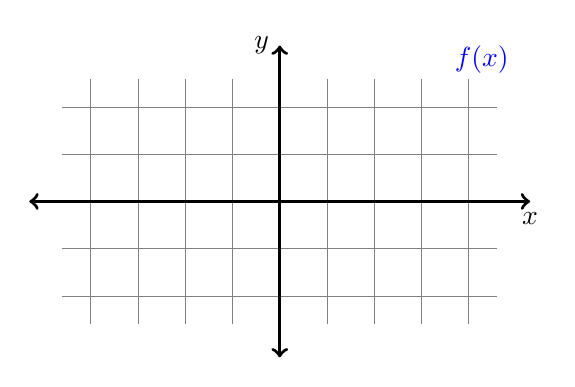
\begin{tikzpicture}[scale=0.6]
\draw[black!50,very thin] (-4.6,-2.6) grid (4.6,2.6);
\draw[very thick,<->] (-5.3,0) -- (5.3,0) node[below] {$x$};
\draw[very thick,<->] (0,-3.3) -- (0,3.3) node[left] {$y$};
\draw[very thick,color=blue,<->] plot[domain=-2.6:3.7,samples=400] function {(x**3 - 2*x**2 - 5*x + 6)/4};
%\draw (-2,0.2) -- (-2,-0.2) node[below] {$-2$};
%\draw  (1,0.2) -- (1,-0.2) node[below] {$1$};
%\draw  (3,0.2) -- (3,-0.2) node[below] {$3$};
%\draw  (-0.2,0.6) -- (0.2,0.6) node[above right] {$1$};
\draw (3.5,3) node[blue, right] {$f(x)$};
\end{tikzpicture}
\end{flushright}

\item Based on the graph above, what are $f(-1)$ and $f(2)$ and $f(3)$?
\vfill


\item A small business sells cupcakes.  The quantity $Q$ of cupcakes demanded by customers depends on how high the business decides to set the price $p$ of a cupcake according to the function:
$$Q(p) = 1800 - 50p^2.$$
Find a formula for the inverse function and explain what it computes. 
\vfill 


\item Let $f(x) = x^2 - 1$ and let $g(y) = \frac{1}{4}y$.  Evaluate the following: $f(g(4))$ and $g(f(3))$.  
\vfill

\item Find a formula for the linear function shown below.
\begin{flushright}
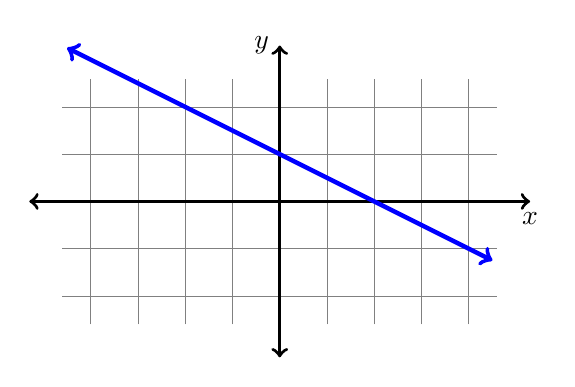
\begin{tikzpicture}[scale=0.6]
\draw[black!50,very thin] (-4.6,-2.6) grid (4.6,2.6);
\draw[very thick,<->] (-5.3,0) -- (5.3,0) node[below] {$x$};
\draw[very thick,<->] (0,-3.3) -- (0,3.3) node[left] {$y$};
\draw[ultra thick,color=blue,<->] (-4.5,3.25) -- (4.5,-1.25);
%\draw (-2,0.2) -- (-2,-0.2) node[below] {$-2$};
%\draw  (1,0.2) -- (1,-0.2) node[below] {$1$};
%\draw  (3,0.2) -- (3,-0.2) node[below] {$3$};
%\draw  (-0.2,0.6) -- (0.2,0.6) node[above right] {$1$};
\end{tikzpicture}
\end{flushright}

\item Find the x-values where the line $y = 2x-1$ intersects the parabola $y = 9 + 5x - x^2$. 
\vfill 

\setcounter{enumCount}{\theenumi}
\end{enumerate}


\end{document}
